\documentclass{article}
\usepackage[utf8]{inputenc}
\usepackage[pdftex]{graphicx} %for embedding images
\usepackage{url} %for proper url entries
\usepackage[bookmarks, colorlinks=false, pdfborder={0 0 0}, pdftitle={Project 01 Report: A Simple Shell}, pdfauthor={Nhut-Nam Le&Dang-Khoa Doan}, pdfsubject={Operating System}, pdfkeywords={report}]{hyperref} %for creating links in the pdf version and other additional pdf attributes, no effect on the printed document
%\usepackage[final]{pdfpages} %for embedding another pdf, remove if not required
\usepackage[utf8]{vietnam}
\usepackage{booktabs}
\usepackage{float}
\usepackage{smartdiagram}
\usepackage{xcolor}
\usepackage[]{algorithm2e}
\usepackage[noend]{algpseudocode}
\usepackage[]{algorithm}
\usepackage{amsmath}
\usepackage{amsfonts}
\usepackage{nicefrac}
\usepackage{amssymb}
\usepackage{arevmath}     % For math symbols
\usesmartdiagramlibrary{additions}
\usepackage[left=3cm, right=3cm, top=2cm, bottom=2cm]{geometry}
\usepackage{parskip}
\usepackage{tikz}
\usepackage{hyperref}
\setlength{\parindent}{15pt}
\setcounter{secnumdepth}{4}
\newcommand{\ra}[1]{\renewcommand{\arraystretch}{#1}}
\newcommand{\code}[1]{\texttt{#1}}
\newcommand\tab[1][1cm]{\hspace*{#1}}
\usepackage{fancyhdr}

\usepackage{pythonhighlight}

\setlength{\headheight}{15.2pt}
\pagestyle{fancy}
\lhead[<even output>]{Hệ điều hành - Operating Systems}
\rhead[<even output>]{A Simple Shell}

\title{report-os-lab-01}
\author{lenam.fithcmus }
\date{October 2020}

%%% Coloring the comment as blue
\newcommand\mycommfont[1]{\footnotesize\ttfamily\textcolor{blue}{#1}}
\algnewcommand\algorithmicforeach{\textbf{for each}}
\algdef{S}[FOR]{ForEach}[1]{\algorithmicforeach\ #1\ \algorithmicdo}
\newcommand{\LoopDo}{\bf loop do}
\SetCommentSty{mycommfont}

\SetKwInput{KwInput}{Input}                % Set the Input
\SetKwInput{KwOutput}{Output}              % set the Output
\let\oldemptyset\emptyset
\let\emptyset\varnothing

\begin{document}

\begin{titlepage}

\begin{center}

% Top of the page

\includegraphics[width=0.3\textwidth]{hcmus.png}\\[0.1in]
\large{ĐẠI HỌC KHOA HỌC TỰ NHIÊN, ĐHQG-HCM\\KHOA CÔNG NGHỆ THÔNG TIN\\BỘ MÔN KHOA HỌC MÁY TÍNH}\\
\normalsize
\vspace{1cm}
\textup{\large {OPERATING SYSTEMS - HỆ ĐIỀU HÀNH}
\vspace{1cm}
\\ 
\Large PROJECT REPORT 01}\\[0.2in]

% Title
\huge \textbf {\\A SIMPLE SHELL}\\[0.2in]
\normalsize
% Lecturers
Giảng viên lý thuyết\\
{\textbf{Trần Trung Dũng}}\\[0.1in]
% Lab Teacher 
Giảng viên thực hành\\
{\textbf{Lê Giang Thanh}}\\[0.2in]
% Submitted by
Nhóm thực hiện \\
\begin{table}[h]
\centering
\begin{tabular}{l l l }\hline \\
Lê Nhựt Nam & 18120061 & 18120061@student.hcmus.edu.vn\\
Đoàn Đăng Khoa & 18120185 & 18120185@student.hcmus.edu.vn\\\\
\hline
\end{tabular}
\end{table}
\vspace{0.2in}

% Date time when written report
\vfill
Tháng 10 năm 2020
\end{center}
\end{titlepage}
\newpage
% End Title


\pagenumbering{roman} %numbering before main content starts
\cleardoublepage
%\pagebreak
\phantomsection
\addcontentsline{toc}{section}{Lời cảm ơn}
\section*{Lời cảm ơn}
\vspace{1.0in}
\begingroup
\setlength{\parindent}{0pt}
Trong quá trình thực hiện đồ án này, em đã nhận được rất nhiều sự giúp đỡ cũng như hỗ trợ từ các thầy cô Trường Đại học Khoa học Tự nhiên, ĐHQG-HCM và các bạn bè trong lớp Hệ Điều Hành - CQ2018 21. Em xin bày tỏ lòng cảm ơn chân thành đến mọi người vì đã giúp đỡ hướng dẫn, chỉ bảo rất tận tình.

Đặc biệt, em xin bày tỏ lòng biết ơn sâu sắc đến các thầy cô khoa Công nghệ Thông tin, cụ thể hơn là thầy Trần Trung Dũng và các thầy hướng dẫn đã giảng dạy rất kĩ lưỡng, cung cấp nhiều slides, tài nguyên học tập cần thiết, tạo điều kiện tốt nhất để bản thân em có thể hoàn thành được đồ án này.

\par


{Đại học Khoa học Tự nhiên, ĐHQG-HCM.}\\
Nhóm thực hiện\\
Tháng 10 năm 2020,\\
\endgroup
\newpage
\tableofcontents
\newpage
\pagenumbering{arabic} %reset numbering to normal for the main content

\section{Tổng quan về đồ án}

\subsection{Mục đích & thiết kế của đồ án}

Với đồ án này, chúng em sẽ cài đặt lại một trình thông dịch lệnh UNIX đơn giản sao chép các chức năng của shell đơn giản (sh), tức sẽ hỗ trợ người dùng thực hiện một số câu lệnh đơn giản.\newline
Các mô hình lệnh sẽ được cài đặt trong chương trình này là: thực thi cơ bản, thực thi dưới nền (background), điều hướng IO (>, <, > >), lịch sử, giao tiếp thông qua pipe. \newline
Hiểu và trình bày được cơ bản về lifetime của một chương trình shell, UNIX fork(), exec(), wait(), dup2() và pipe() system calls.\newline
Chương trình thiết kế trên vòng lặp vô hạn, sử dụng dấu nhắc lệnh có định dạng "<current day> <space> <current time> <space> <username>:<current directory working> >", được thiết kế gồm 4 phần chính:
-	Executing command in a child process.
-	Creating a history feature.
-	Redirecting input and output (">" and  "<")
-	Communication via a pipe.

\subsection{Bảng bảng đánh giá}
\begin{table*}[h]\centering
\ra{1.3}
\begin{tabular}{p{3cm}p{4cm}p{3cm}l}\toprule
\textbf{Trình bày} & \textbf{Lệnh} & \textbf{Người thực hiện} &\textbf{Điểm tự đánh giá} \tabularnewline
\midrule
& Các lệnh đơn giản với các tiến trình con & Nhựt Nam, Đăng Khoa & 30 \tabularnewline
& Lệnh đơn giản với  & Đăng Khoa & 5  \tabularnewline
& Chuyển hướng Input & Nhựt Nam & 15  \tabularnewline
& Chuyển hướng Outnput & Đăng Khoa & 15 \tabularnewline
& Thực thi hai lệnh với một pipe & Đăng Khoa & 15 \tabularnewline
Code Quality, Comments, Report the result in file (screenshot) & & Nhựt Nam & 20  \tabularnewline
Tổng điểm & & & 100  \tabularnewline
\bottomrule
\end{tabular}
\end{table*}

\section{Shell là gì?}

Shell là chương trình người dùng đặc biệt, cung cấp giao diện cho người dùng sử dụng các dịch vụ hệ điều hành. Shell chấp nhận các lệnh có thể đọc được từ người dùng và chuyển đổi chúng thành thứ mà kernel có thể hiểu được.\newline
Theo linuxcommand.org shell được định nghĩa: " the shell is a program that takes commands from the keyboard and gives them to the operating system to perform"\newline

\section{Chu trình sống của một chương trình Shell}
1. Khởi động chương trình shell.\newline
2. Đọc input từ người dùng.\newline
3. Paser lệnh được nhập từ người dùng. Nếu là lệnh "exit" hoặc "quit" (Tùy quy định thoát chương trình của người lập trình) thì thoát chương trình shell.\newline
4. Thực thi lệnh và trả kết quả cho người dùng.\newline
5. Quay lại bước 2.

\section{Các lệnh system calls có dùng trong đồ án}
\subsection{Lệnh fork()}

\begin{figure}[H]
\centering
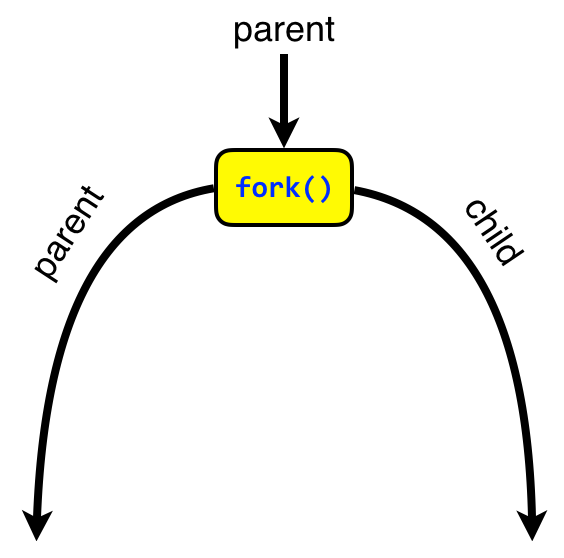
\includegraphics[width=0.5\textwidth]{fork.png}
\caption{Minh họa lệnh fork()}
\end{figure}

\subsection{Lệnh exec(), wait(), exit()}
execl - execv - execle - execve - execlp - execvp

\begin{figure}[H]
\centering
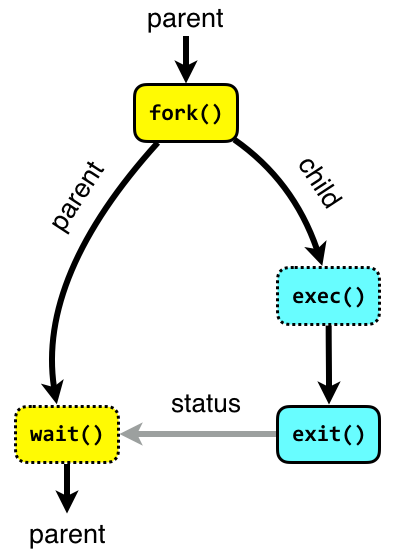
\includegraphics[width=0.5\textwidth]{fork-exec-exit-wait.png}
\caption{Minh họa lệnh fork() - exec() - exit() - wait()}
\end{figure}

\subsection{Lệnh pipe()}
\begin{figure}[H]
\centering
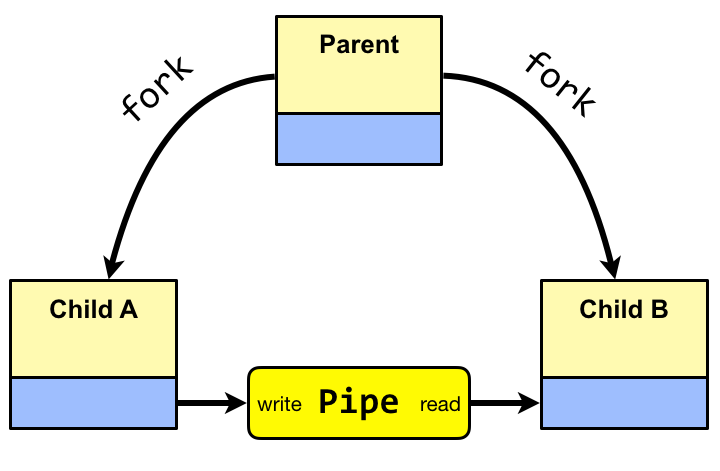
\includegraphics[width=0.5\textwidth]{pipe_1.png}
\caption{Minh họa pipe()}
\end{figure}



\section{Đọc input người dùng}

\subsection{Parse command}
\begin{lstlisting}[language=C]
void parse_command(char *input_string, char **argv, int *is_background) 
\end{lstlisting}

\subsection{Parse redirect command}
Hàm kiểm tra
\begin{lstlisting}[language=C]
int is_redirect(char **argv) 
\end{lstlisting}
Hàm parse
\begin{lstlisting}[language=C]
void parse_redirect(char **argv, char **redirect_argv, int redirect_index)
\end{lstlisting}

\subsection{Parse pipe command}
Hàm kiểm tra
\begin{lstlisting}[language=C]
int is_pipe(char **argv)
\end{lstlisting}
Hàm parse
\begin{lstlisting}[language=C]
void parse_pipe(char **argv, char **child01_argv, 
char **child02_argv, int pipe_index)
\end{lstlisting}

\section{Thực thi lệnh trong một tiến trình con}

\begin{figure}[H]
\centering
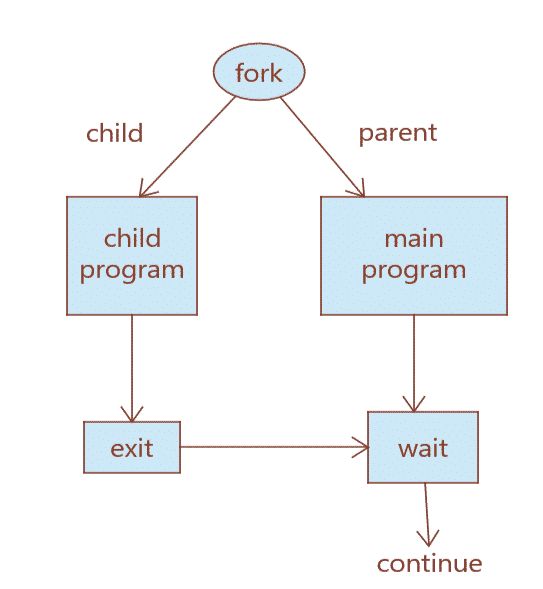
\includegraphics[width=0.5\textwidth]{Executing Command in a Child Process.png}
\caption{Thực thi lệnh trong một tiến trình con}
\end{figure}

\section{Tính năng Lịch sử với "!!"}


\section{Chuyển hướng đầu vào và đầu ra}

\subsection{Chuyển hướng đầu vào}
\begin{lstlisting}[language=C]
void exec_child_overwrite_from_file(char **argv, char **dir)
\end{lstlisting}


\subsection{Chuyển hướng đầu ra}
\begin{lstlisting}[language=C]
void exec_child_overwrite_to_file(char **argv, char **dir)
\end{lstlisting}


\section{Giao tiếp qua Pipe}
\begin{lstlisting}[language=C]
void exec_child_pipe(char **argv_in, char **argv_out)
\end{lstlisting}

\begin{figure}[H]
\centering
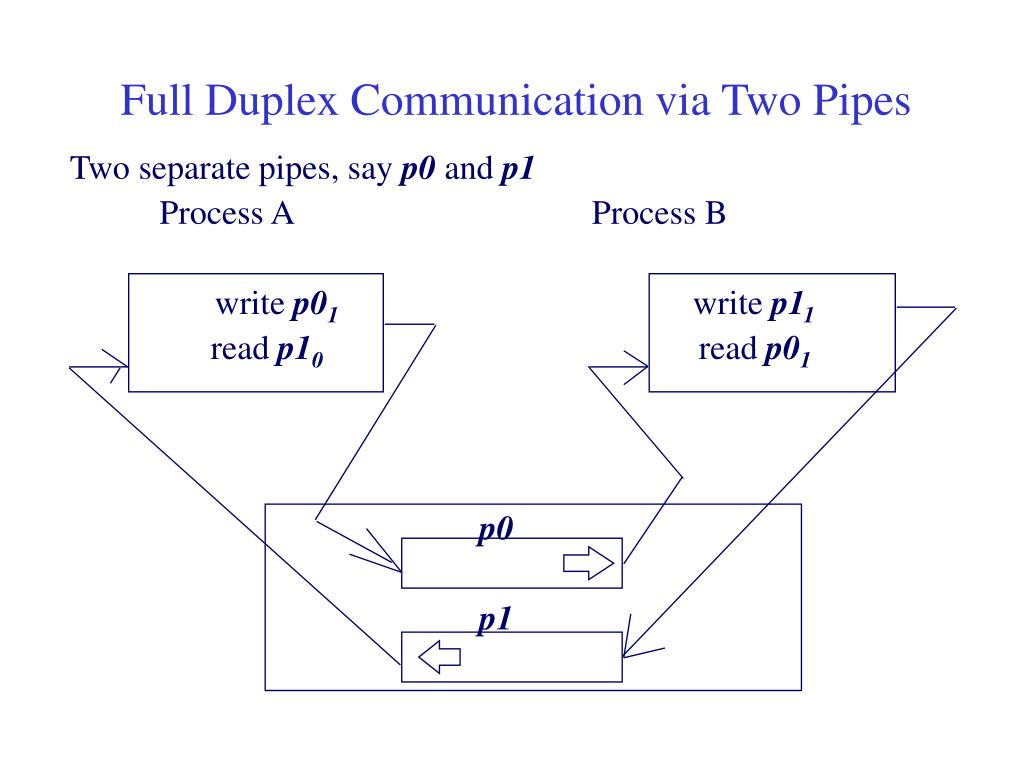
\includegraphics[width=0.98\textwidth]{pipe.jpg}
\caption{Minh họa cách giao tiếp thông qua Pipe}
\end{figure}

\section{Kiểm thử}

Yêu cầu: Linux Debian (có thể dùng Ubuntu, Zorin, Xbuntu, Kubuntu, ...), Make (4.2.1), GNU GCC Compiler >= 7.5.0)\newline
Lib: readline library "sudo apt-get install libreadline-dev"\newline
Các build project:\newline
Bước 01: cd vào thư mục src của project\newline
Bước 02: Mở termial bằng cách nhấn tổ hợp phím Ctrl + ALt + T, gõ command "make build" để build project, sau đó gõ command "make run" để run chương trình simple shell\newline

\subsection{Thực thi lệnh cơ bản}

\begin{figure}[H]
\centering
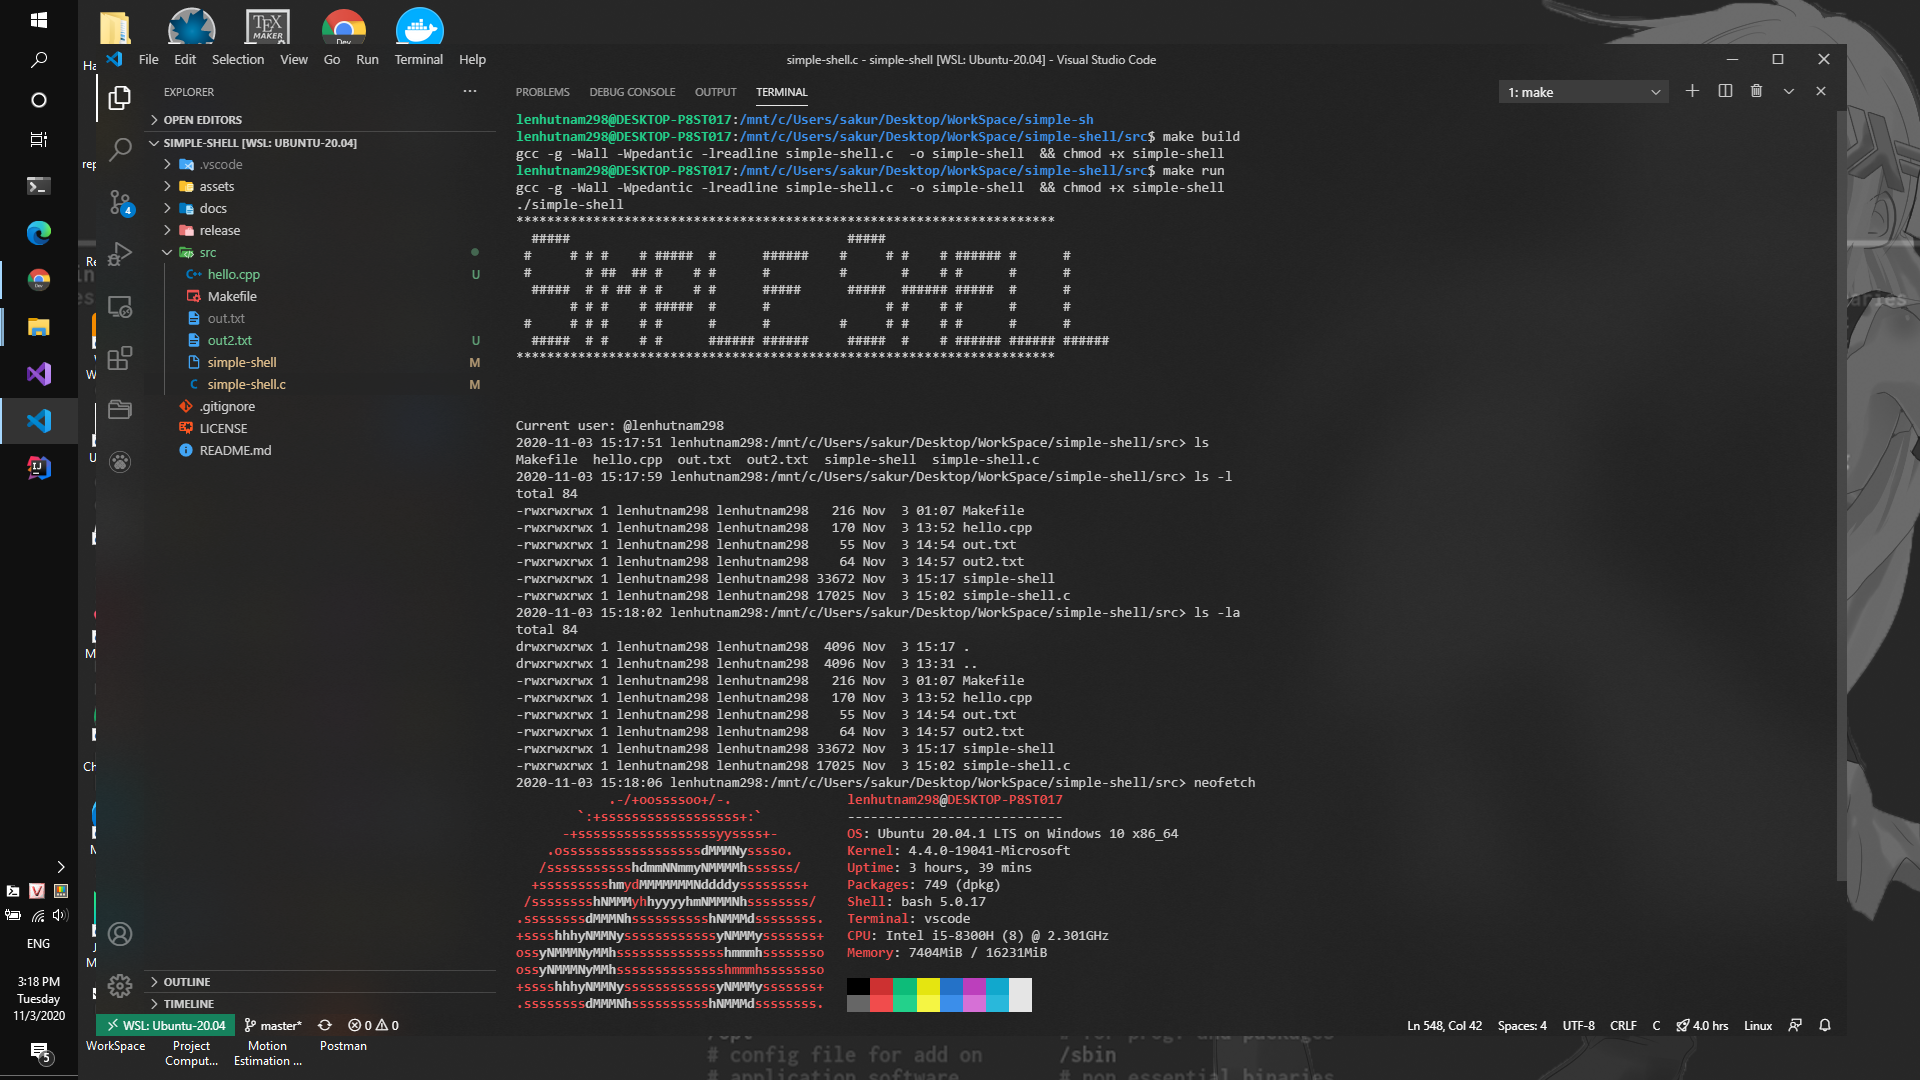
\includegraphics[width=0.98\textwidth]{wsl_simple_command.png}
\caption{Thực thi lệnh đơn giản trên WSL - Ubuntu 20.04}
\end{figure}

\begin{figure}[H]
\centering
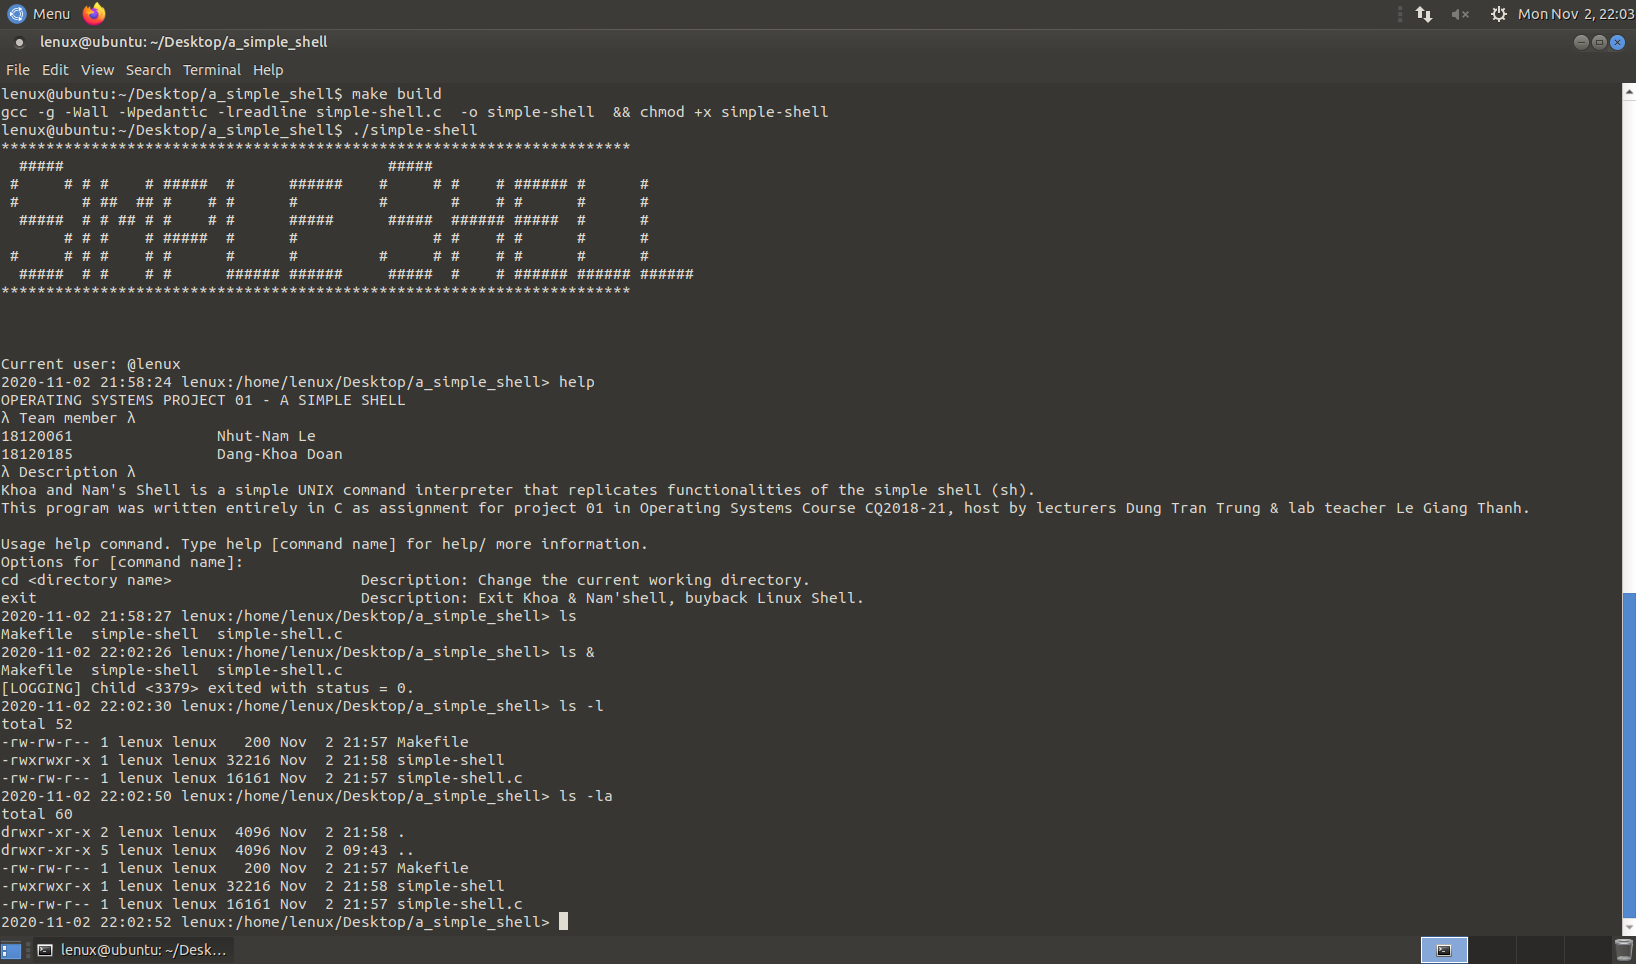
\includegraphics[width=0.98\textwidth]{virtual_machine_executing_command_in_child_process.png}
\caption{Thực thi lệnh đơn giản trên Virtual Machine - Ubuntu 18.04}
\end{figure}

\subsection{Thực thi lệnh dưới nền}

\begin{figure}[H]
\centering
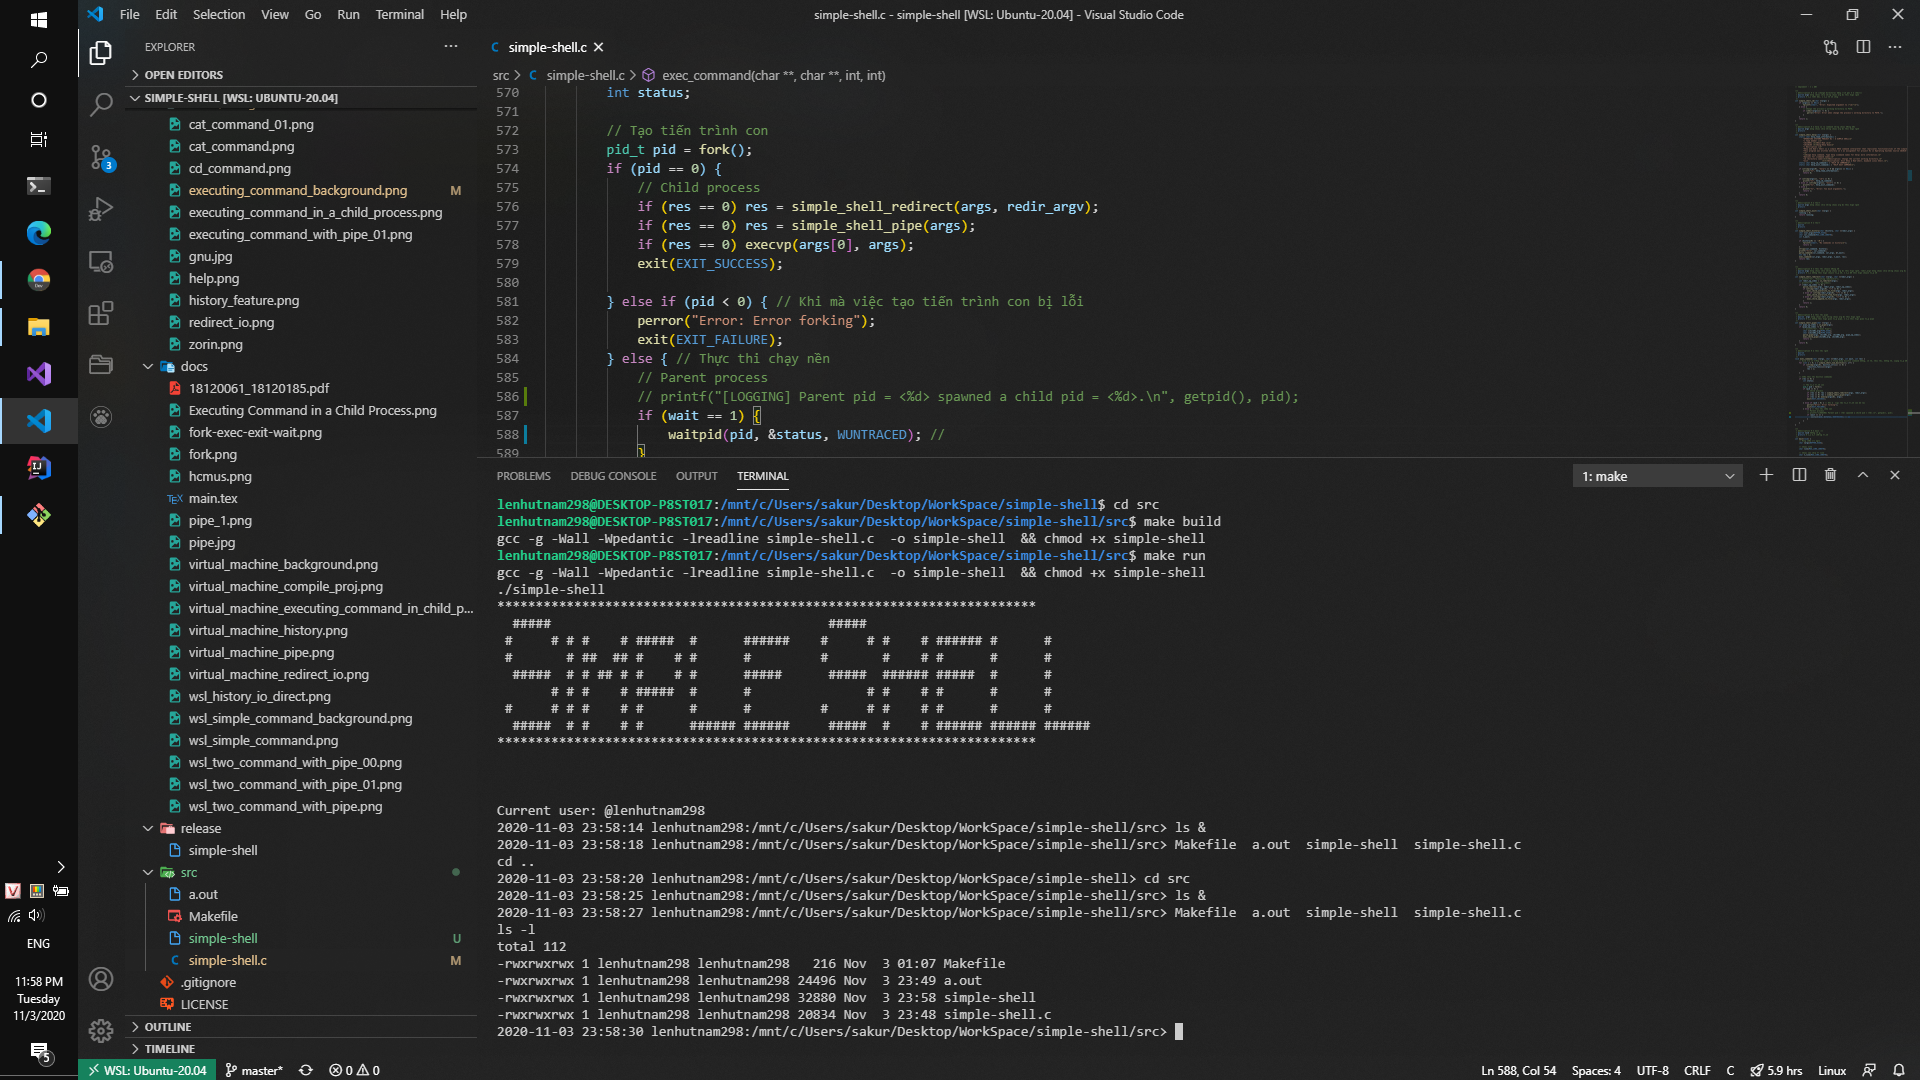
\includegraphics[width=0.98\textwidth]{wsl_simple_command_background.png}
\caption{Thực thi lệnh dưới nền và chức năng lịch sn trên WSL - Ubuntu 20.04}
\end{figure}

\begin{figure}[H]
\centering
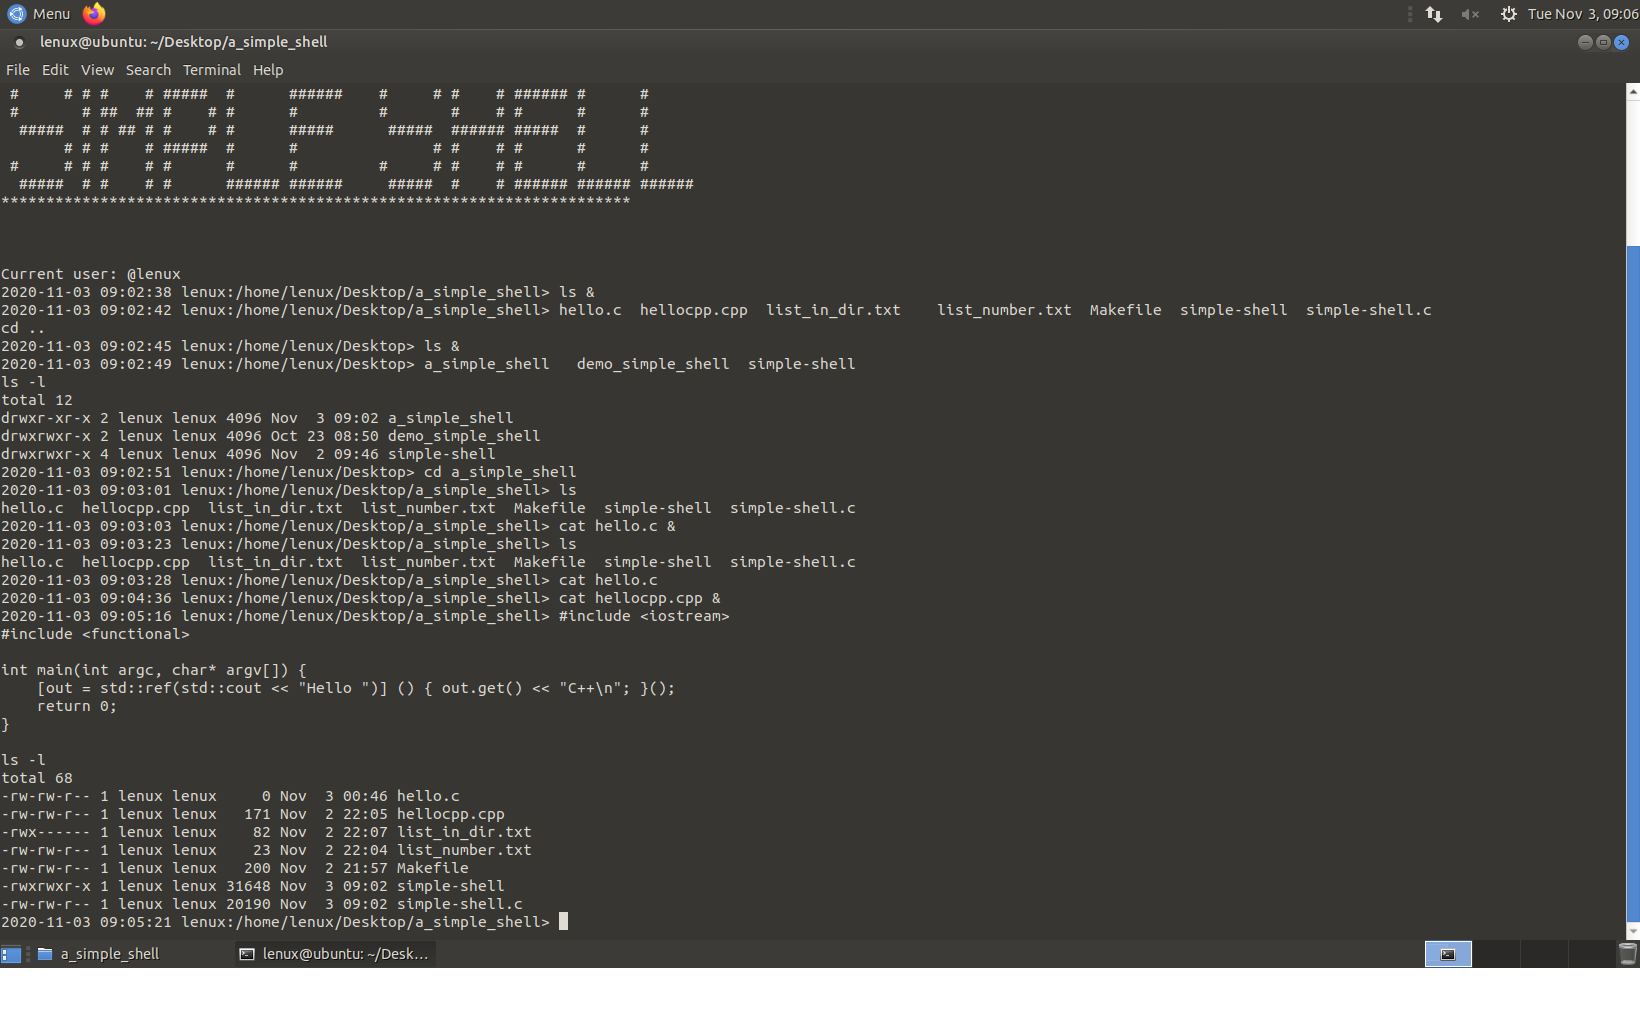
\includegraphics[width=0.98\textwidth]{virtual_machine_background.png}
\caption{Thực thi lệnh dưới nền trên Virtual Machine - Ubuntu 18.04}
\end{figure}

\subsection{Chuyển hướng đầu vào/ đầu ra và chức năng lịch sử}

\begin{figure}[H]
\centering
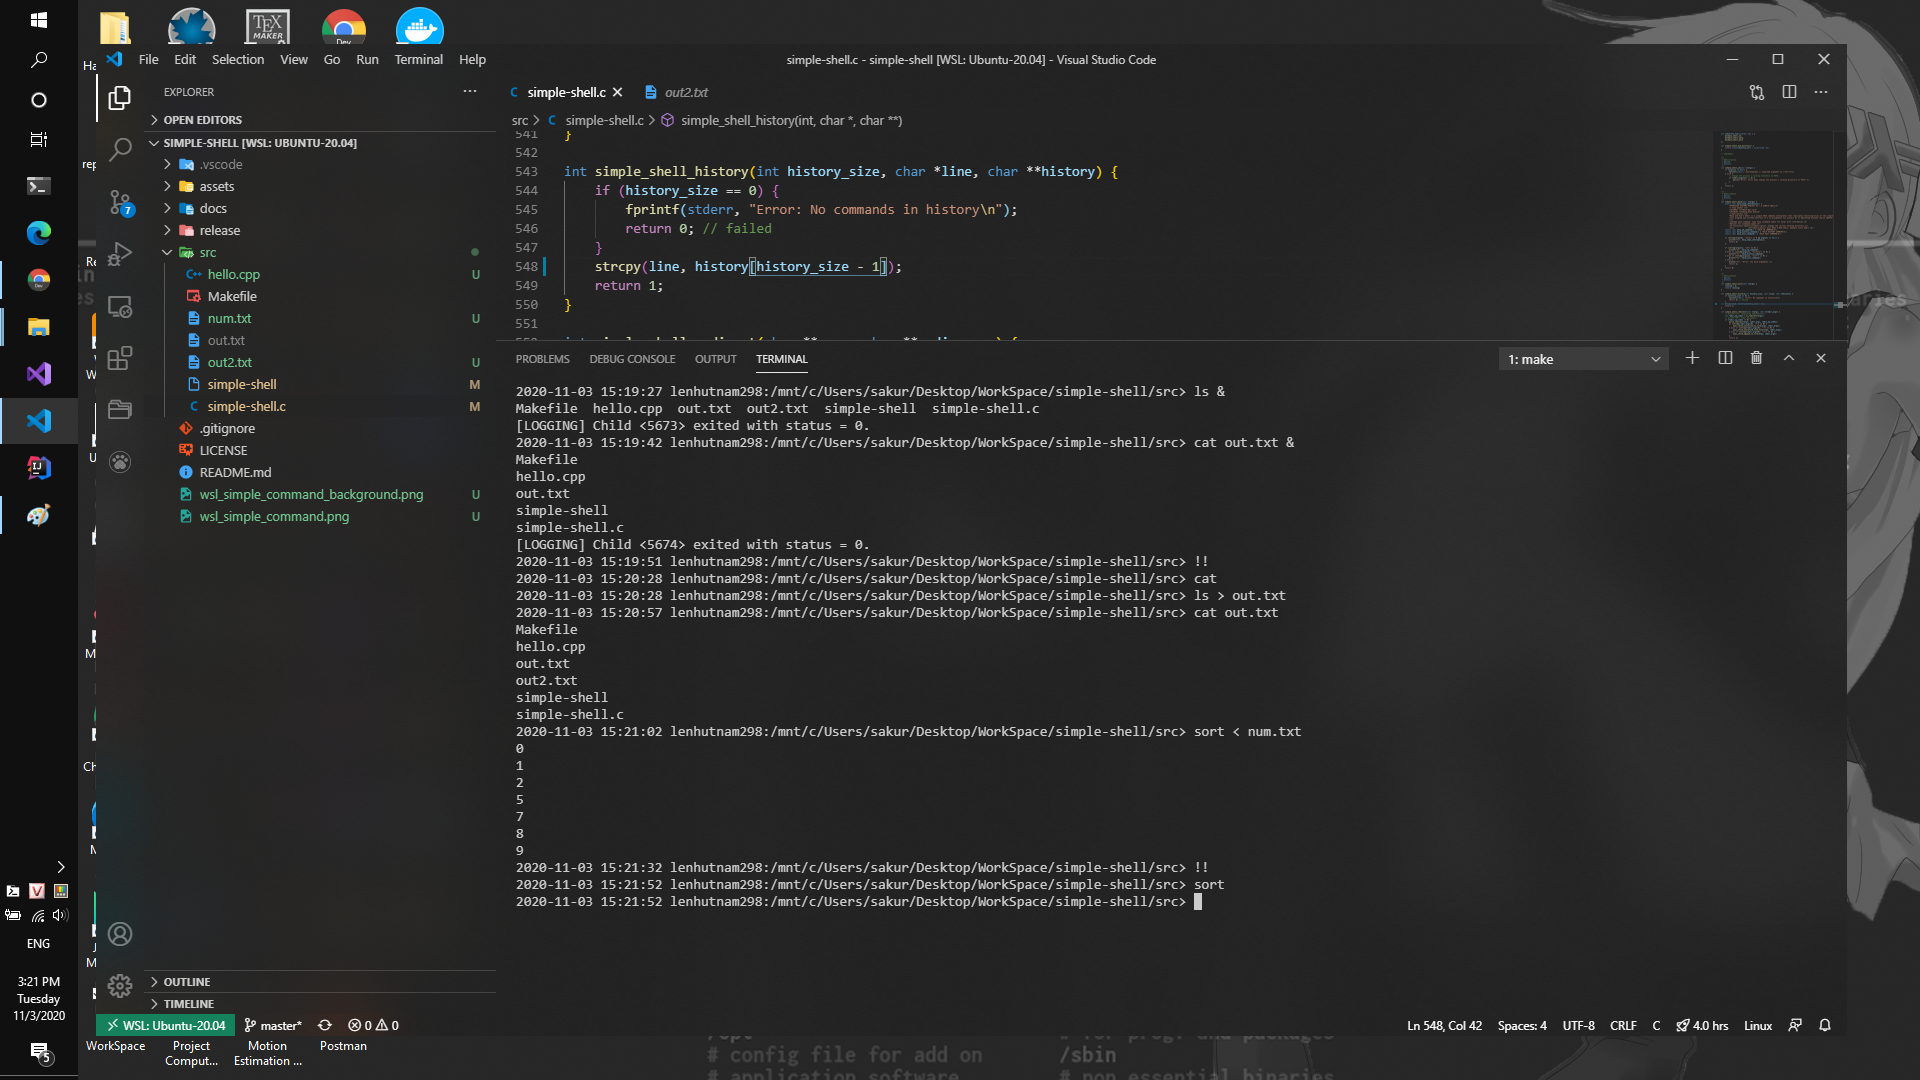
\includegraphics[width=0.98\textwidth]{wsl_history_io_direct.png}
\caption{Chuyển hướng đầu vào/ đầu ra và chức năng lịch sử trên WSL - Ubuntu 20.04}
\end{figure}

\begin{figure}[H]
\centering
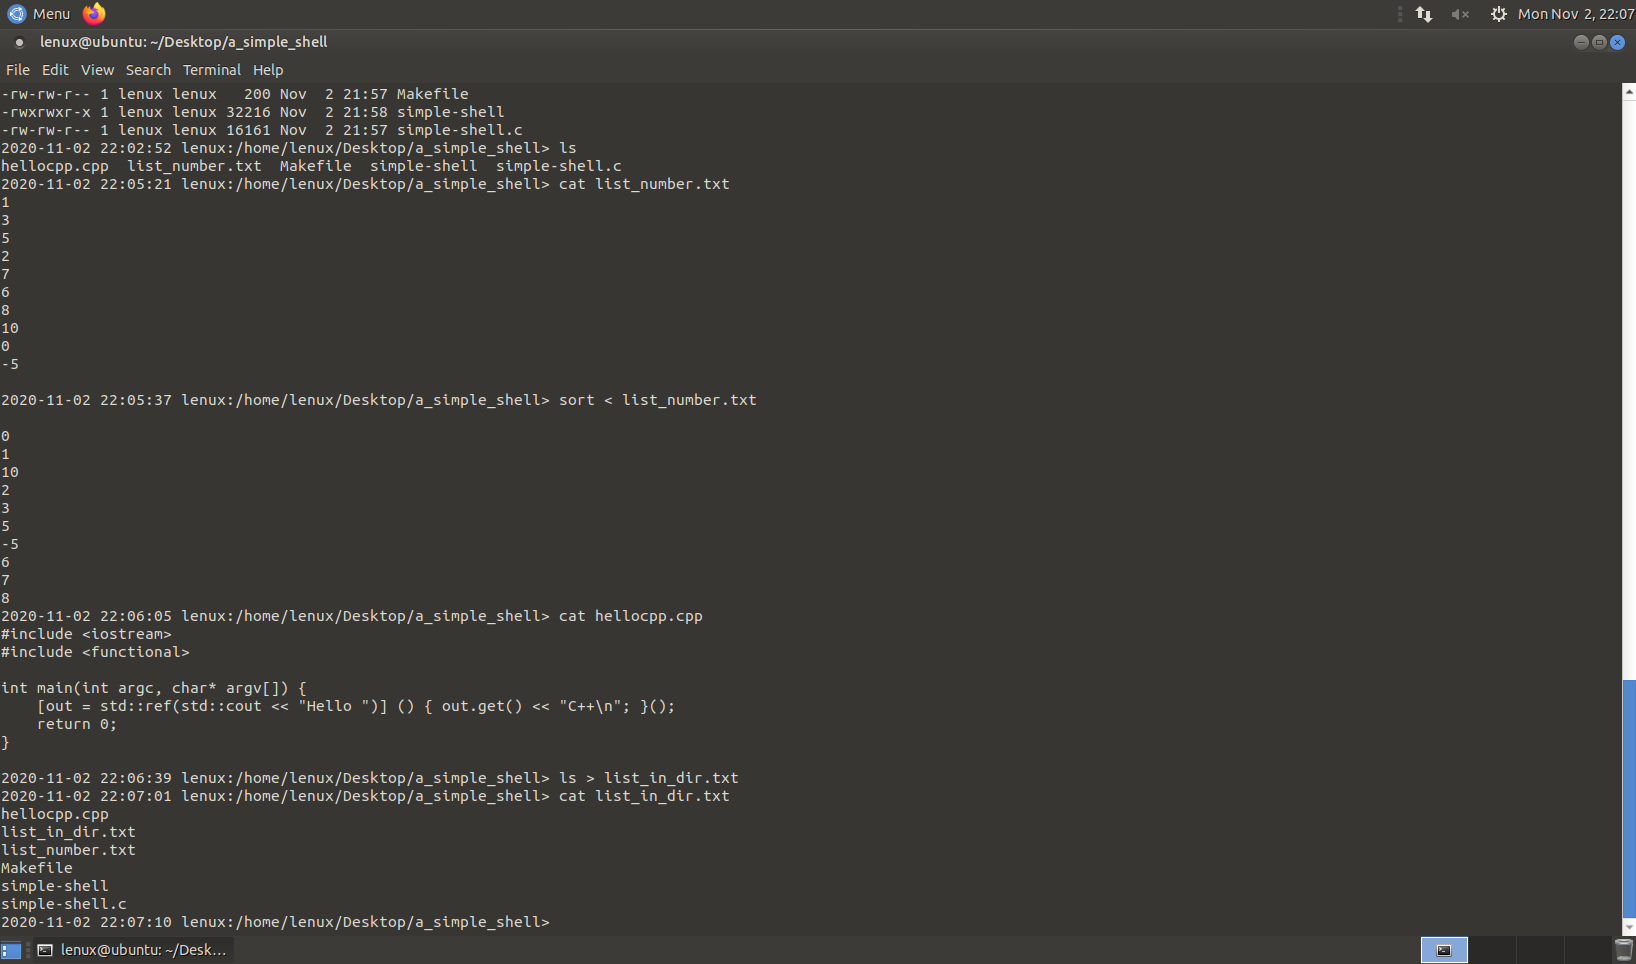
\includegraphics[width=0.98\textwidth]{virtual_machine_redirect_io.png}
\caption{Chuyển hướng đầu vào/ đầu ra trên Virtual Machine - Ubuntu 18.04}
\end{figure}

\subsection{Giao tiếp hai lệnh thông qua Pipe}

\begin{figure}[H]
\centering
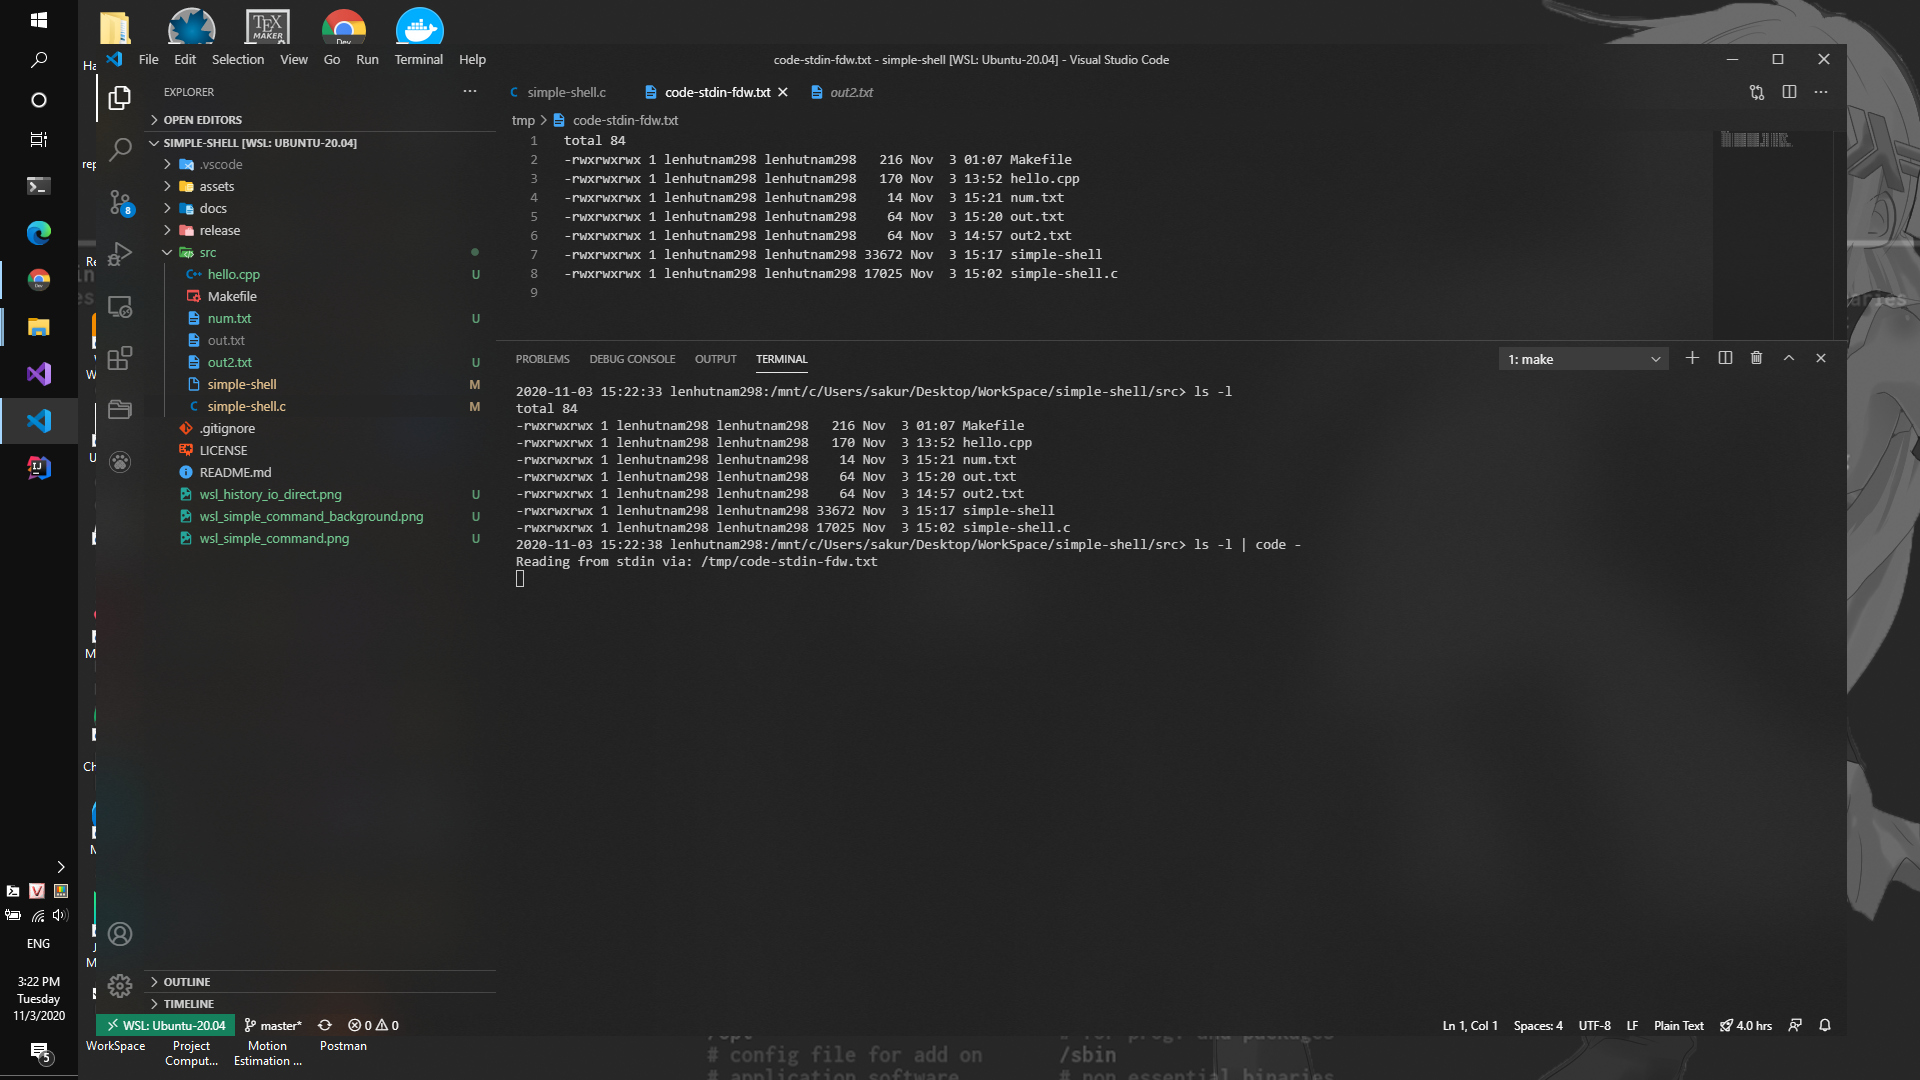
\includegraphics[width=0.98\textwidth]{wsl_two_command_with_pipe.png}
\caption{Test: ls -l | code- }
\end{figure}


\begin{figure}[H]
\centering
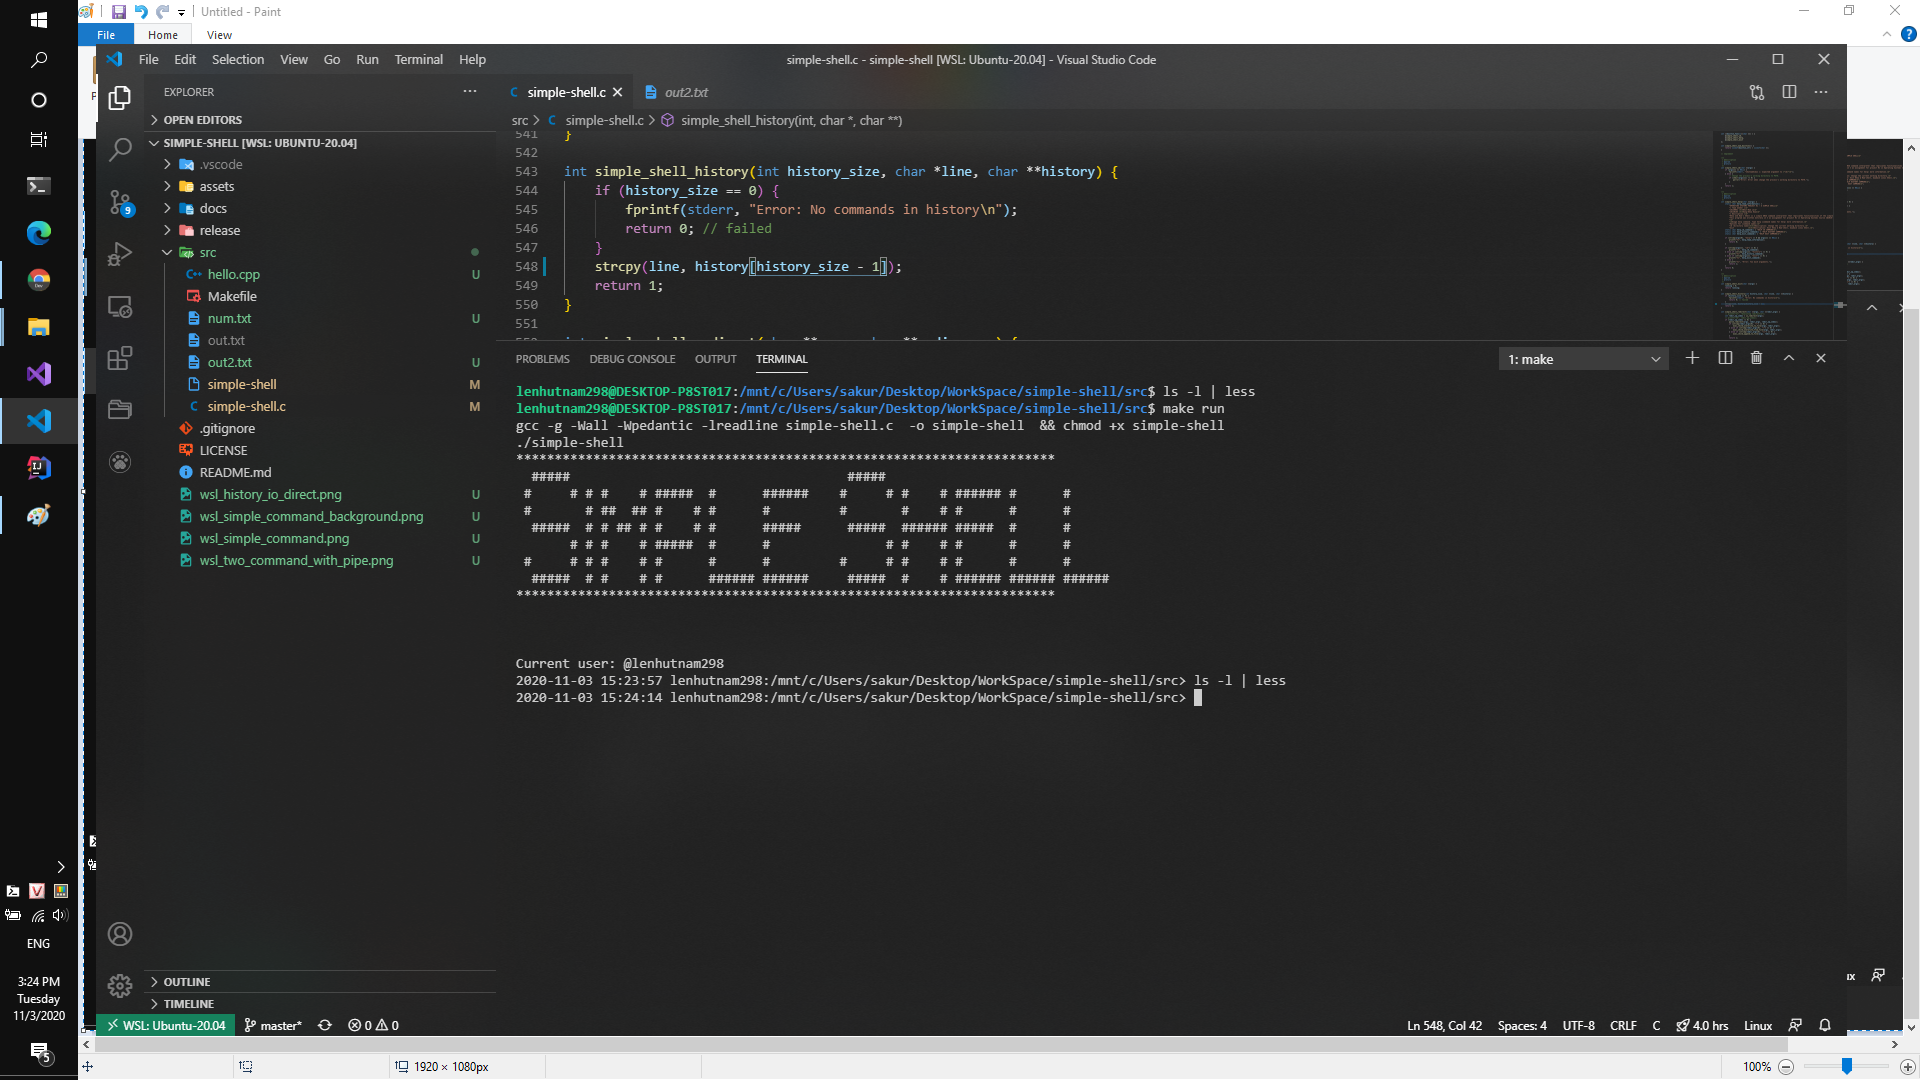
\includegraphics[width=0.98\textwidth]{wsl_two_command_with_pipe_01.png}
\caption{Test: ls -l | less}
\end{figure}

\begin{figure}[H]
\centering
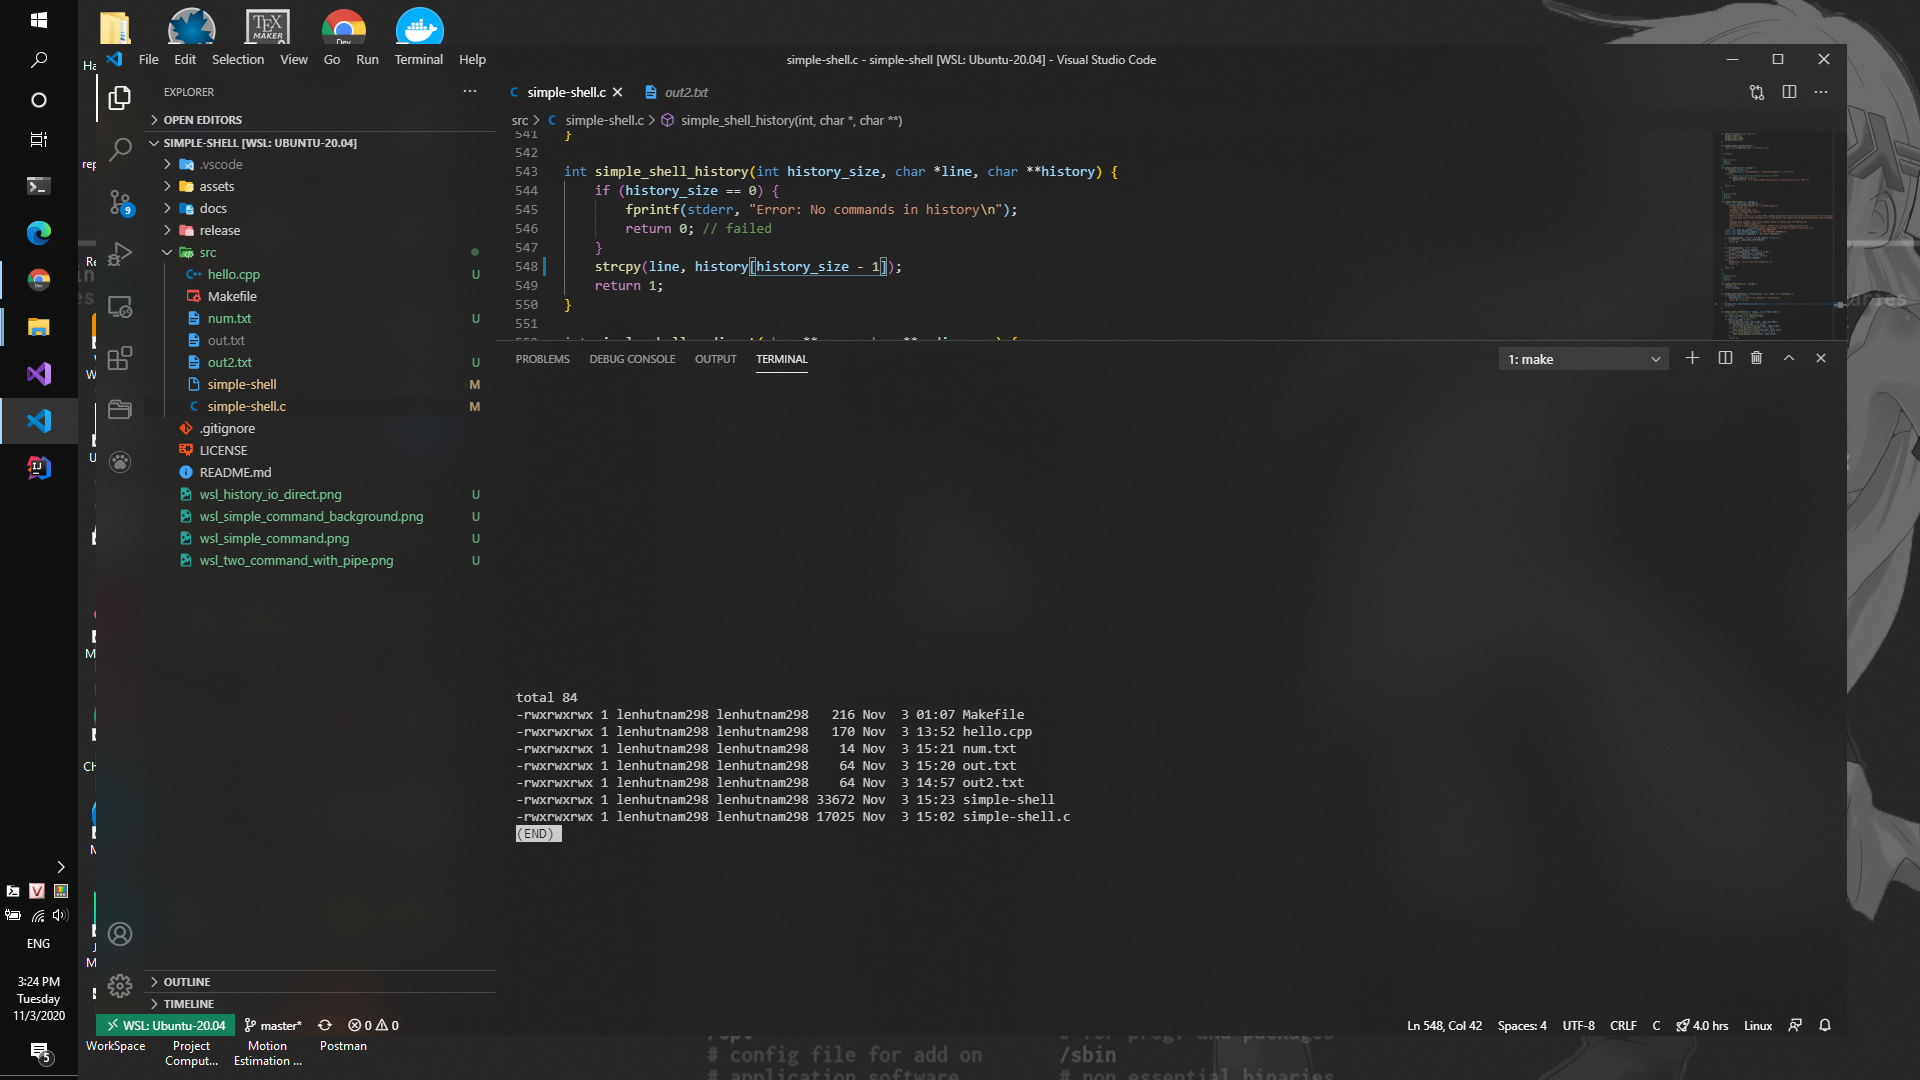
\includegraphics[width=0.98\textwidth]{wsl_two_command_with_pipe_00.png}
\caption{Test: ls -l | less}
\end{figure}

\begin{figure}[H]
\centering
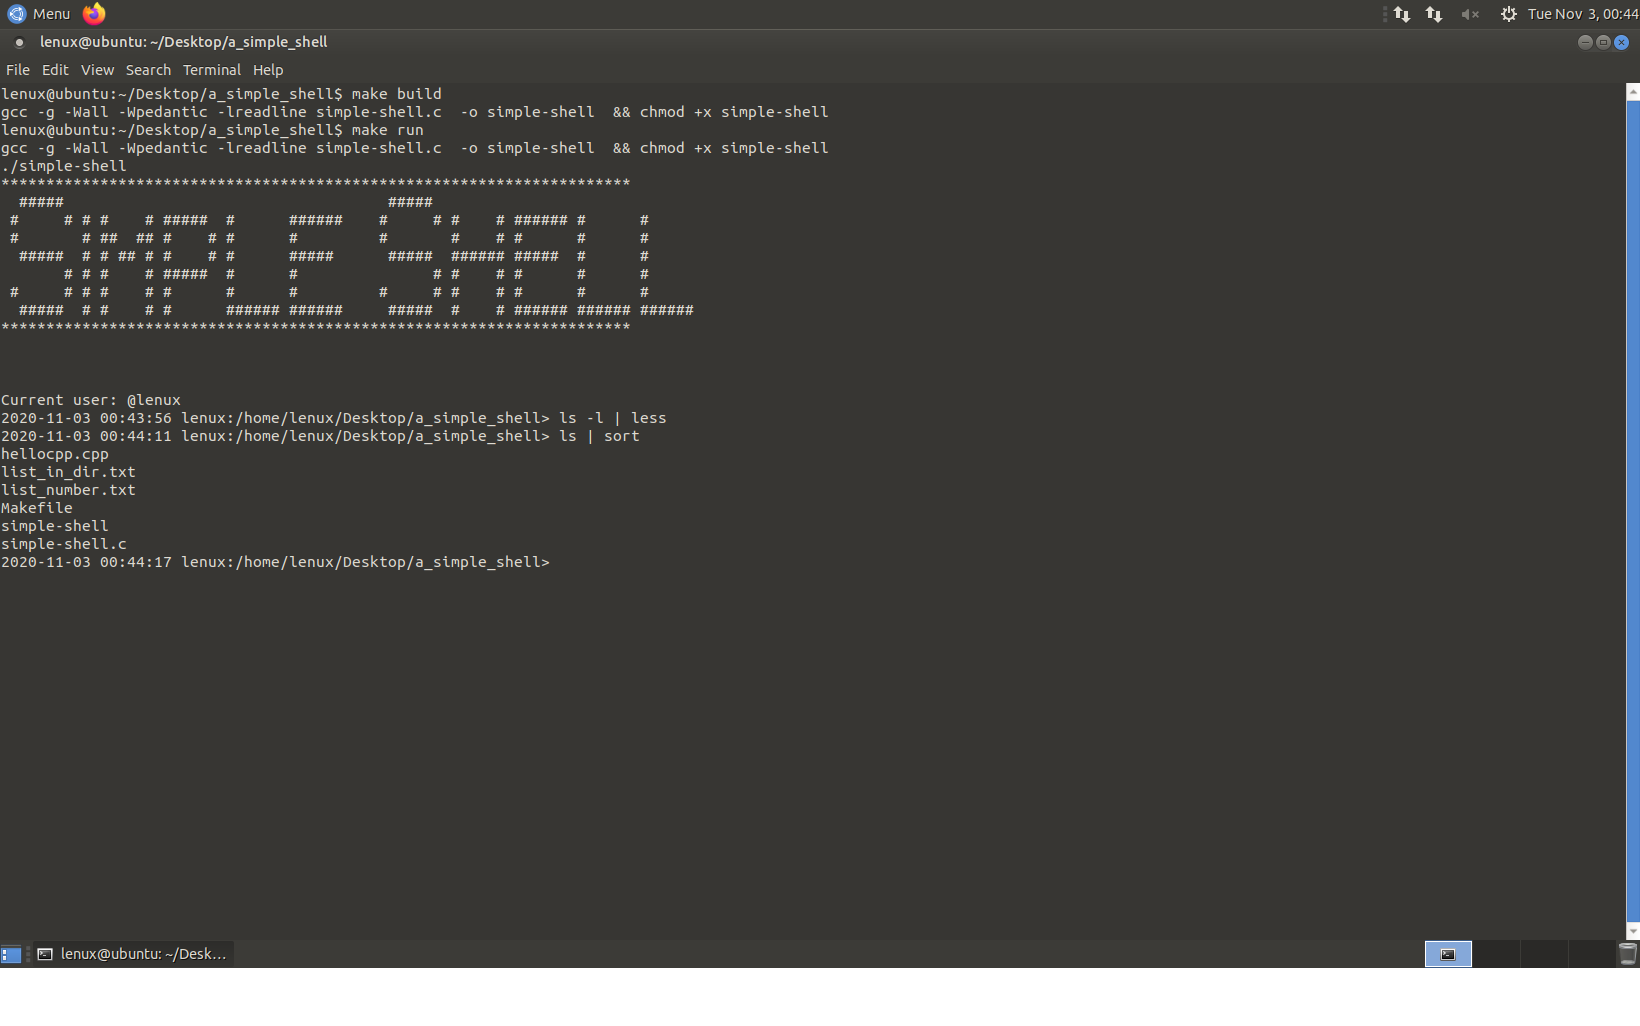
\includegraphics[width=0.98\textwidth]{virtual_machine_pipe.png}
\caption{Test thực thi Pipe trên VM Ubuntu 18.04}
\end{figure}

\section{Tài liệu tham khảo}
[1] \href{https://linux.die.net/man/2/}{Linux man pages - System calls}\newline
[2] \href{https://www.youtube.com/watch?v=k6TTj4C0LF0}{EnthusiastiCon - Stefanie Schirmer “OMG building a shell in 10 minutes”} \newline
\end{document}
